% !TEX root = ./article.tex

\documentclass[spanish]{article}

\usepackage{mystyle}
\usepackage{myvars}
\usepackage{mylinearprogramming}



%-----------------------------

\begin{document}

	\maketitle % Insert title

	\thispagestyle{fancy} % All pages have headers and footers


%-----------------------------
%	ABSTRACT
%-----------------------------

	\begin{abstract}
		\noindent [TODO ]
	\end{abstract}

%-----------------------------
%	TEXT
%-----------------------------

	\section{Introducción}
	\label{sec:intro}

		\paragraph{}
		[TODO ]

	\section{Problema del Viajero (TSP)}

		\paragraph{}
		[TODO ]

		\subsection{Estrategia Exacta}

			\paragraph{}
			[TODO ]

		\subsection{Estrategia Greedy}

			\paragraph{}
			[TODO ]


		\subsection{Estrategia 2-OPT}

			\paragraph{}
			[TODO ]

		\subsection{Estrategia GRASP}

			\paragraph{}
			[TODO ]

		\subsection{Estrategia Simulated Anneling}

			\paragraph{}
			[TODO ]

	\section{Problema del Viajero con Ventana de Tiempo (TSPTW)}

		\paragraph{}
		[TODO ]


	\section{Resolución de Problemas}

		\subsection{burma14}

			\paragraph{}
			[TODO ]

		\subsection{br17}

			\paragraph{}
			[TODO ]

		\subsection{n21\_1}

			\paragraph{}
			[TODO ]

			\begin{table}
				\centering
				\begin{tabu}{ | c | c | p{.65\linewidth} |}
					\hline
			   	\bfseries Método & \bfseries Distancia & \bfseries Camino
			    \csvreader[head to column names]{../results/csv/results-n21_1.csv}{}
			    {\\\hline\method&\distance&\path}
					\\\hline
		    \end{tabu}
				\caption{Soluciones para el conjunto de datos \emph{n21\_1}}
				\label{table:sol-n21_1}
			\end{table}

		\subsection{n21\_2}

			\paragraph{}
			[TODO ]

			\begin{table}
				\centering
				\begin{tabu}{ | c | c | p{.65\linewidth} |}
					\hline
			   	\bfseries Método & \bfseries Distancia & \bfseries Camino
			    \csvreader[head to column names]{../results/csv/results-n21_2.csv}{}
			    {\\\hline\method&\distance&\path}
					\\\hline
		    \end{tabu}
				\caption{Soluciones para el conjunto de datos \emph{n21\_2}}
				\label{table:sol-n21_1}
			\end{table}

		\subsection{n21\_3}

			\paragraph{}
			[TODO ]

			\begin{table}
				\centering
				\begin{tabu}{ | c | c | p{.65\linewidth} |}
					\hline
			   	\bfseries Método & \bfseries Distancia & \bfseries Camino
			    \csvreader[head to column names]{../results/csv/results-n21_3.csv}{}
			    {\\\hline\method&\distance&\path}
					\\\hline
		    \end{tabu}
				\caption{Soluciones para el conjunto de datos \emph{n21\_3}}
				\label{table:sol-n21_1}
			\end{table}

		\subsection{n21\_4}

			\paragraph{}
			[TODO ]
			\begin{table}
				\centering
				\begin{tabu}{ | c | c | p{.65\linewidth} |}
					\hline
			   	\bfseries Método & \bfseries Distancia & \bfseries Camino
			    \csvreader[head to column names]{../results/csv/results-n21_4.csv}{}
			    {\\\hline\method&\distance&\path}
					\\\hline
		    \end{tabu}
				\caption{Soluciones para el conjunto de datos \emph{n21\_4}}
				\label{table:sol-n21_1}
			\end{table}

		\subsection{n21\_5}

			\paragraph{}
			[TODO ]

			\begin{table}
				\centering
				\begin{tabu}{ | c | c | p{.65\linewidth} |}
					\hline
			   	\bfseries Método & \bfseries Distancia & \bfseries Camino
			    \csvreader[head to column names]{../results/csv/results-n21_5.csv}{}
			    {\\\hline\method&\distance&\path}
					\\\hline
		    \end{tabu}
				\caption{Soluciones para el conjunto de datos \emph{n21\_5}}
				\label{table:sol-n21_1}
			\end{table}

		\subsection{tsp\_60\_1}

			\paragraph{}
			[TODO ]

			\begin{table}
				\centering
				\begin{tabu}{ | c | c | p{.65\linewidth} |}
					\hline
			   	\bfseries Método & \bfseries Distancia & \bfseries Camino
			    \csvreader[head to column names]{../results/csv/results-tsp_60_1.csv}{}
			    {\\\hline\method&\distance&\path}
					\\\hline
		    \end{tabu}
				\caption{Soluciones para el conjunto de datos \emph{tsp\_60\_1}}
				\label{table:sol-n21_1}
			\end{table}


			\begin{figure}[h]
				\centering
				\begin{subfigure}{.4\textwidth}
					\centering
					%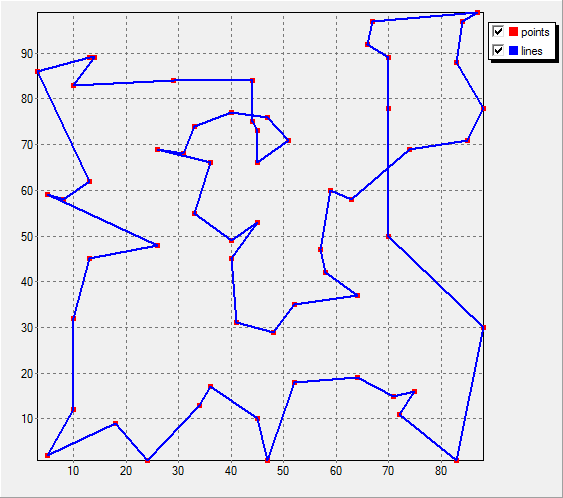
\includegraphics[width=\linewidth]{results-tsp_60_1-exact}
					\caption{Solución \emph{Exacta} para \emph{tsp\_60\_1}}
				\end{subfigure} \
				\begin{subfigure}{.4\textwidth}
					\centering
					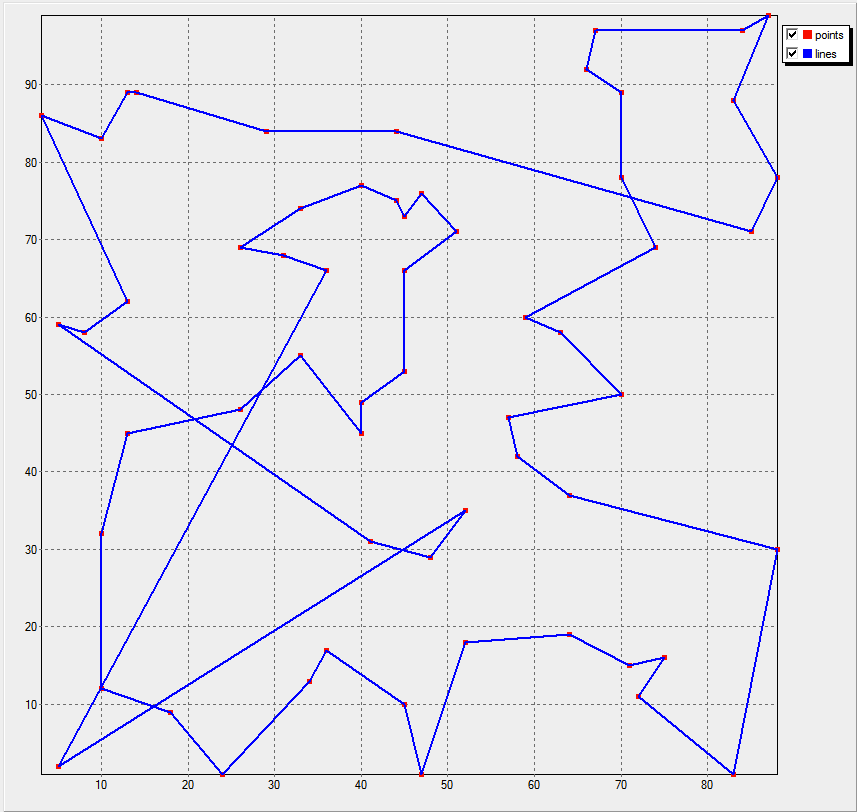
\includegraphics[width=\linewidth]{results-tsp_60_1-greedy}
					\caption{Solución \emph{Greedy} para \emph{tsp\_60\_1}}
				\end{subfigure} \\
				\begin{subfigure}{.4\textwidth}
					\centering
					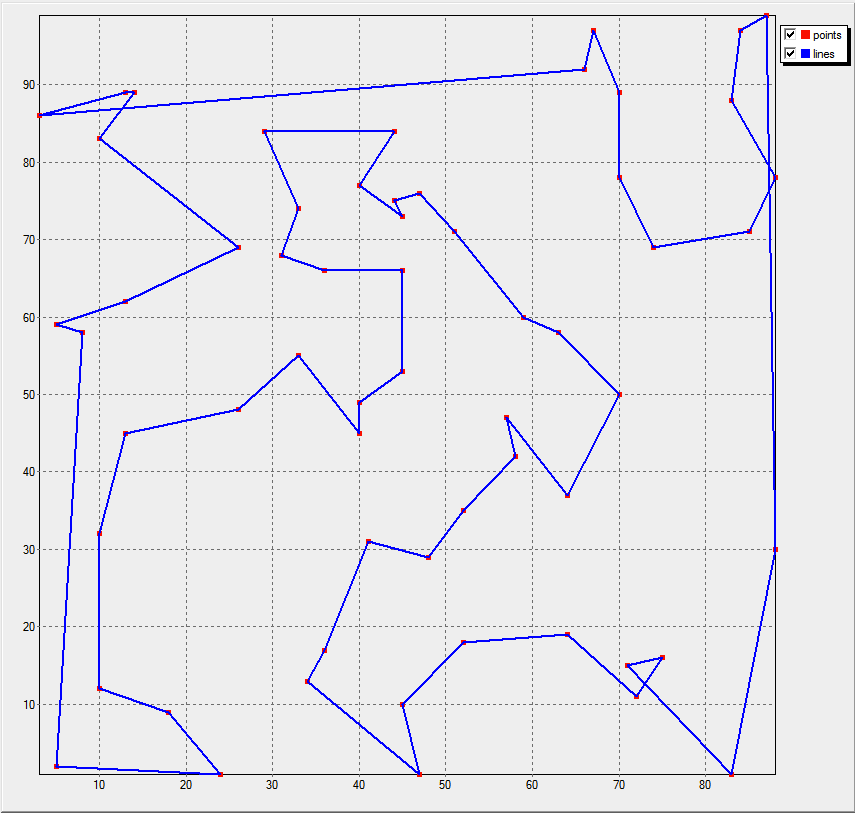
\includegraphics[width=\linewidth]{results-tsp_60_1-opt}
					\caption{Solución \emph{2-opt} para \emph{tsp\_60\_1}}
				\end{subfigure} \
				\begin{subfigure}{.4\textwidth}
					\centering
					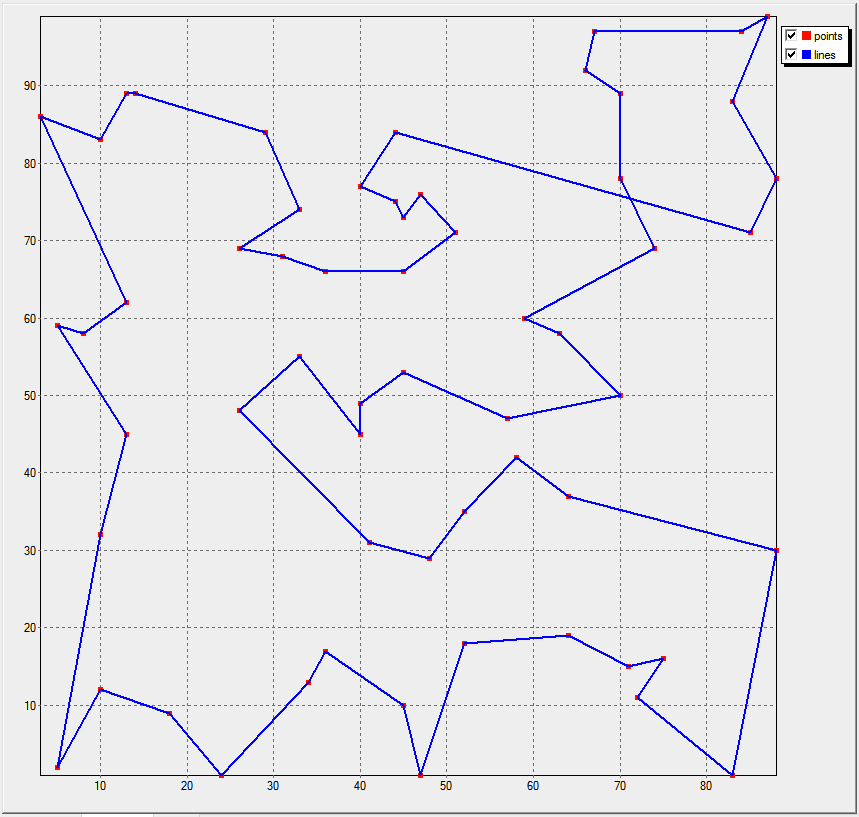
\includegraphics[width=\linewidth]{results-tsp_60_1-grasp}
					\caption{Solución \emph{GRASP} para \emph{tsp\_60\_1}}
				\end{subfigure} \\
				\begin{subfigure}{.4\textwidth}
					\centering
					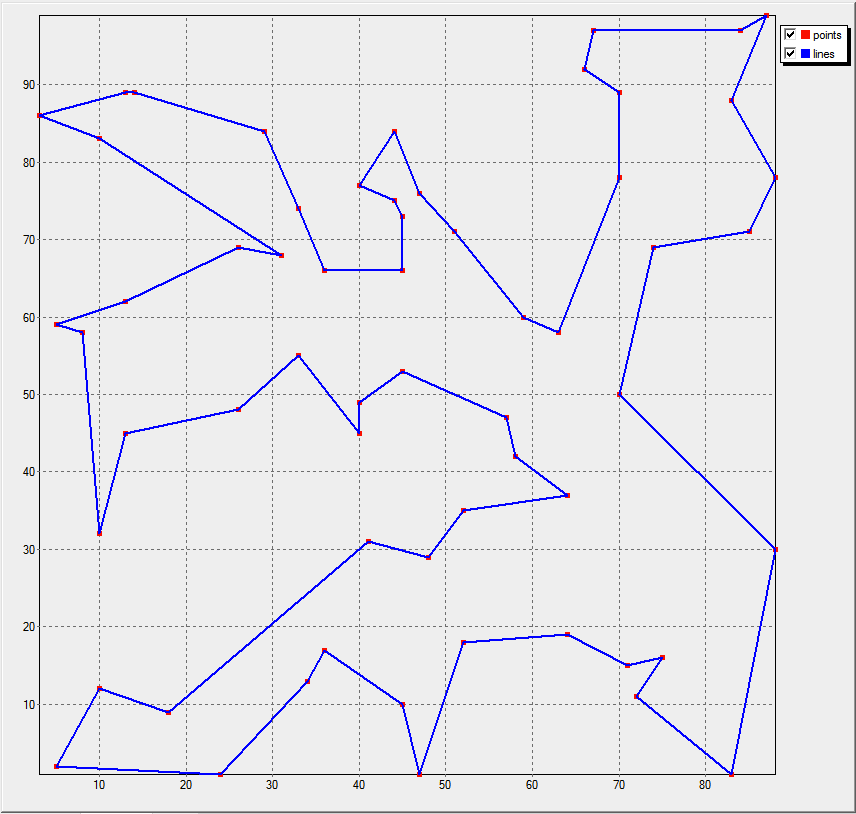
\includegraphics[width=\linewidth]{results-tsp_60_1-sa}
					\caption{Solución \emph{Simulated Anneling} para \emph{tsp\_60\_1}}
				\end{subfigure}
				\caption{Representación gráfica de las distintas soluciones para el conjunto de datos \emph{tsp\_60\_1}}
				\label{fig:sol-tsp_60_1}
			\end{figure}


		\subsection{tsp\_60\_2}

			\paragraph{}
			[TODO ]

			\begin{table}
				\centering
				\begin{tabu}{ | c | c | p{.65\linewidth} |}
					\hline
			   	\bfseries Método & \bfseries Distancia & \bfseries Camino
			    \csvreader[head to column names]{../results/csv/results-tsp_60_2.csv}{}
			    {\\\hline\method&\distance&\path}
					\\\hline
		    \end{tabu}
				\caption{Soluciones para el conjunto de datos \emph{tsp\_60\_2}}
				\label{table:sol-n21_1}
			\end{table}

			\begin{figure}[h]
				\centering
				\begin{subfigure}{.4\textwidth}
					\centering
					%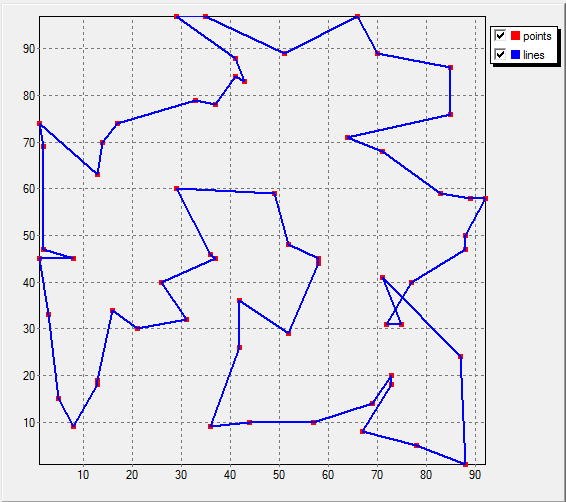
\includegraphics[width=\linewidth]{results-tsp_60_2-exact}
					\caption{Solución \emph{Exacta} para \emph{tsp\_60\_2}}
				\end{subfigure} \
				\begin{subfigure}{.4\textwidth}
					\centering
					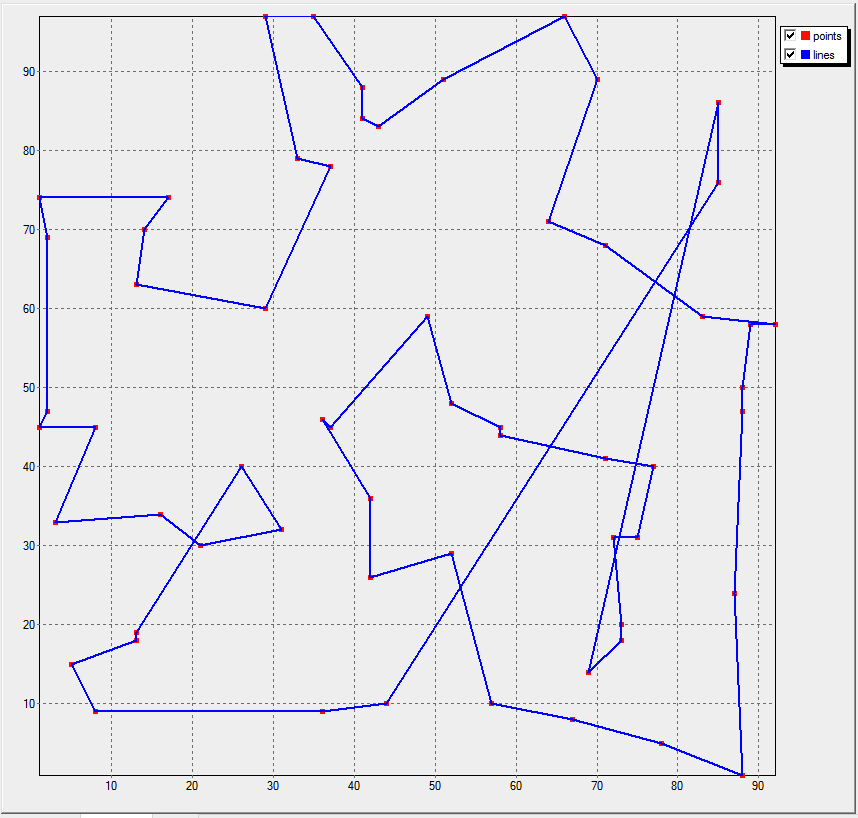
\includegraphics[width=\linewidth]{results-tsp_60_2-greedy}
					\caption{Solución \emph{Greedy} para \emph{tsp\_60\_2}}
				\end{subfigure} \\
				\begin{subfigure}{.4\textwidth}
					\centering
					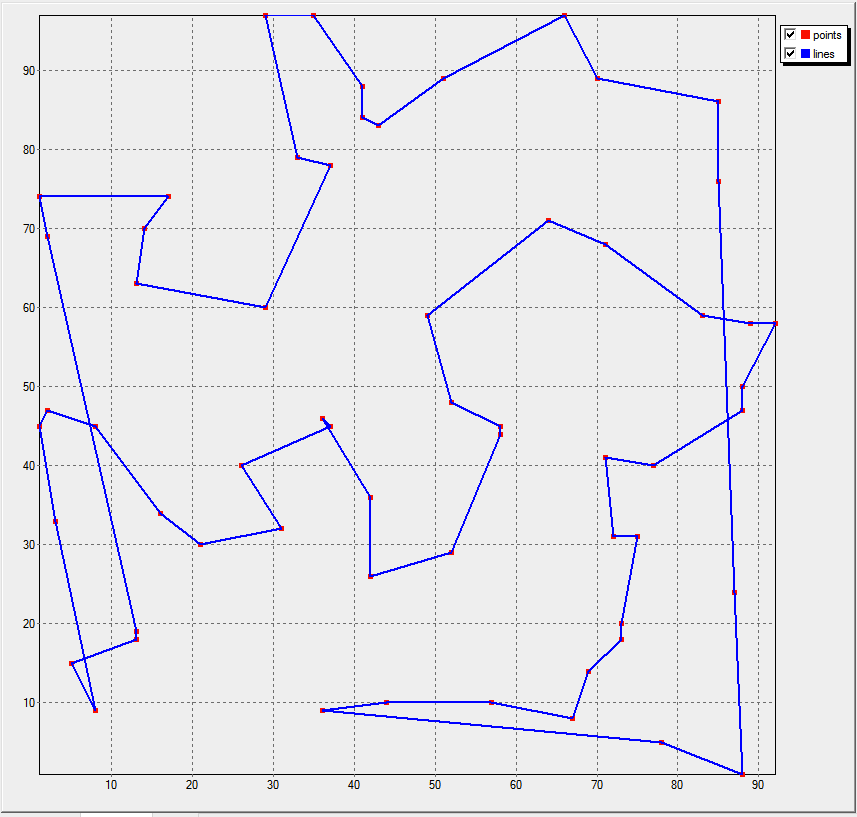
\includegraphics[width=\linewidth]{results-tsp_60_2-opt}
					\caption{Solución \emph{2-opt} para \emph{tsp\_60\_2}}
				\end{subfigure} \
				\begin{subfigure}{.4\textwidth}
					\centering
					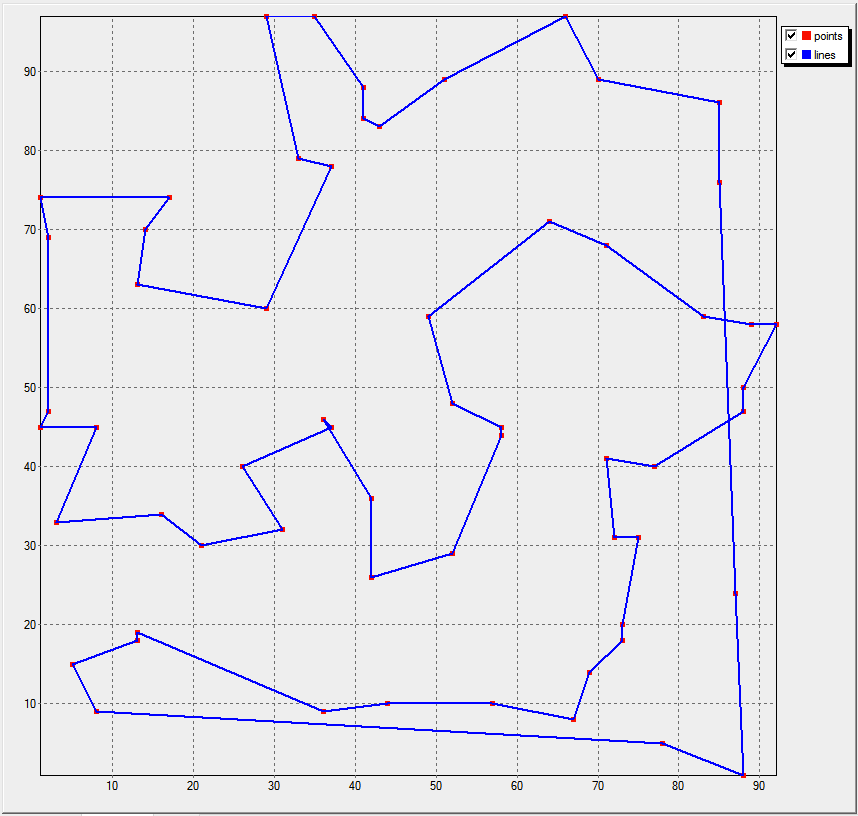
\includegraphics[width=\linewidth]{results-tsp_60_2-grasp}
					\caption{Solución \emph{GRASP} para \emph{tsp\_60\_2}}
				\end{subfigure} \\
				\begin{subfigure}{.4\textwidth}
					\centering
					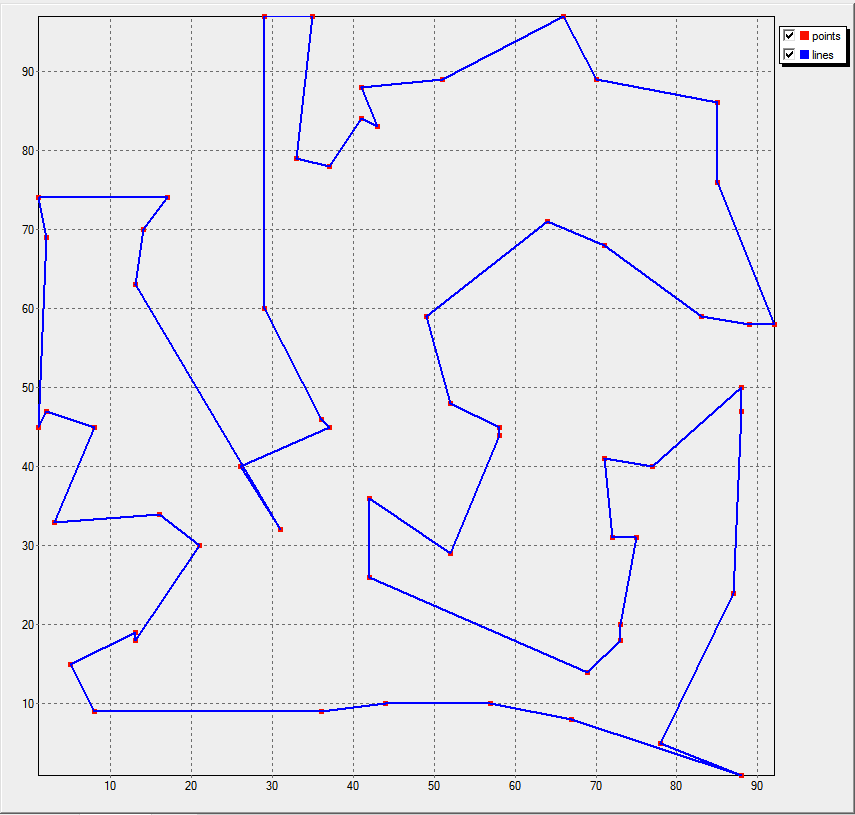
\includegraphics[width=\linewidth]{results-tsp_60_2-sa}
					\caption{Solución \emph{Simulated Anneling} para \emph{tsp\_60\_2}}
				\end{subfigure}
				\caption{Representación gráfica de las distintas soluciones para el conjunto de datos \emph{tsp\_60\_2}}
				\label{fig:sol-tsp_60_2}
			\end{figure}

		\subsection{tsp\_60\_3}

			\paragraph{}
			[TODO ]

			\begin{table}
				\centering
				\begin{tabu}{ | c | c | p{.65\linewidth} |}
					\hline
			   	\bfseries Método & \bfseries Distancia & \bfseries Camino
			    \csvreader[head to column names]{../results/csv/results-tsp_60_3.csv}{}
			    {\\\hline\method&\distance&\path}
					\\\hline
		    \end{tabu}
				\caption{Soluciones para el conjunto de datos \emph{tsp\_60\_3}}
				\label{table:sol-n21_1}
			\end{table}

			\begin{figure}[h]
				\centering
				\begin{subfigure}{.4\textwidth}
					\centering
					%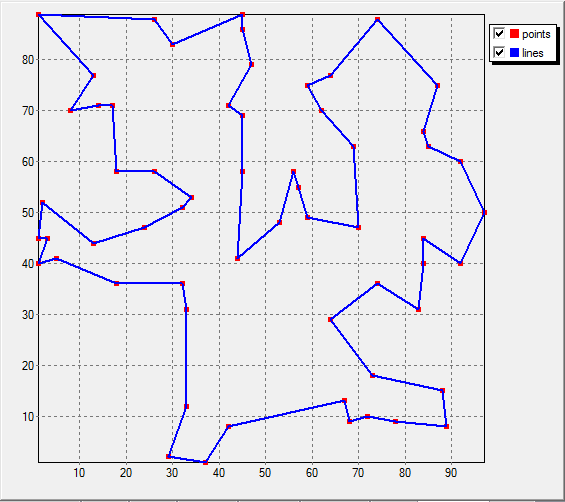
\includegraphics[width=\linewidth]{results-tsp_60_3-exact}
					\caption{Solución \emph{Exacta} para \emph{tsp\_60\_3}}
				\end{subfigure} \
				\begin{subfigure}{.4\textwidth}
					\centering
					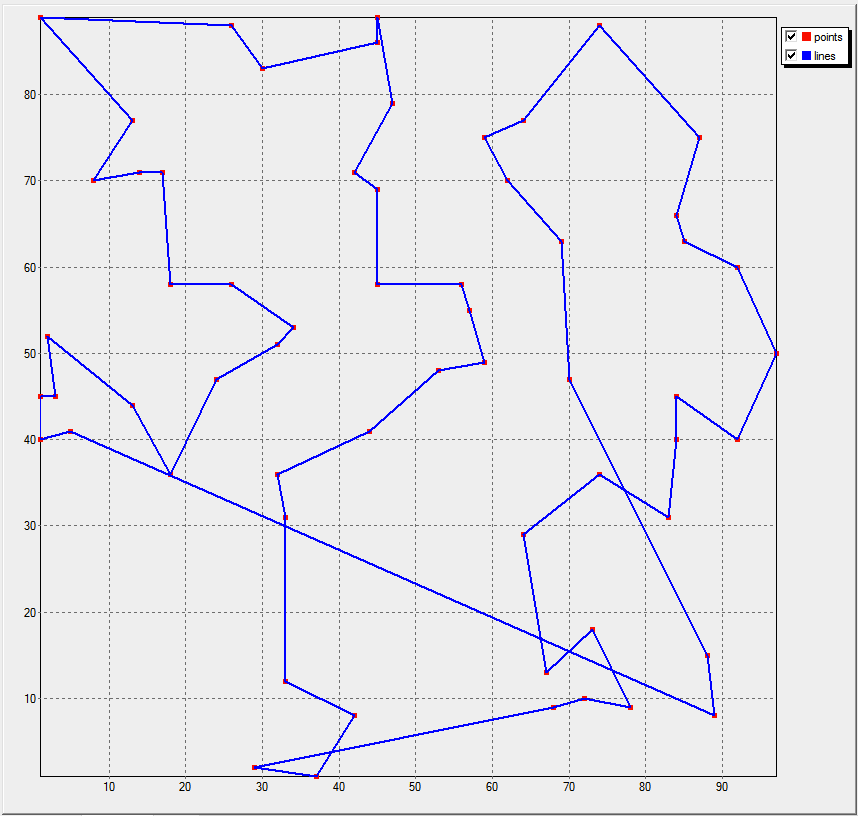
\includegraphics[width=\linewidth]{results-tsp_60_3-greedy}
					\caption{Solución \emph{Greedy} para \emph{tsp\_60\_3}}
				\end{subfigure} \\
				\begin{subfigure}{.4\textwidth}
					\centering
					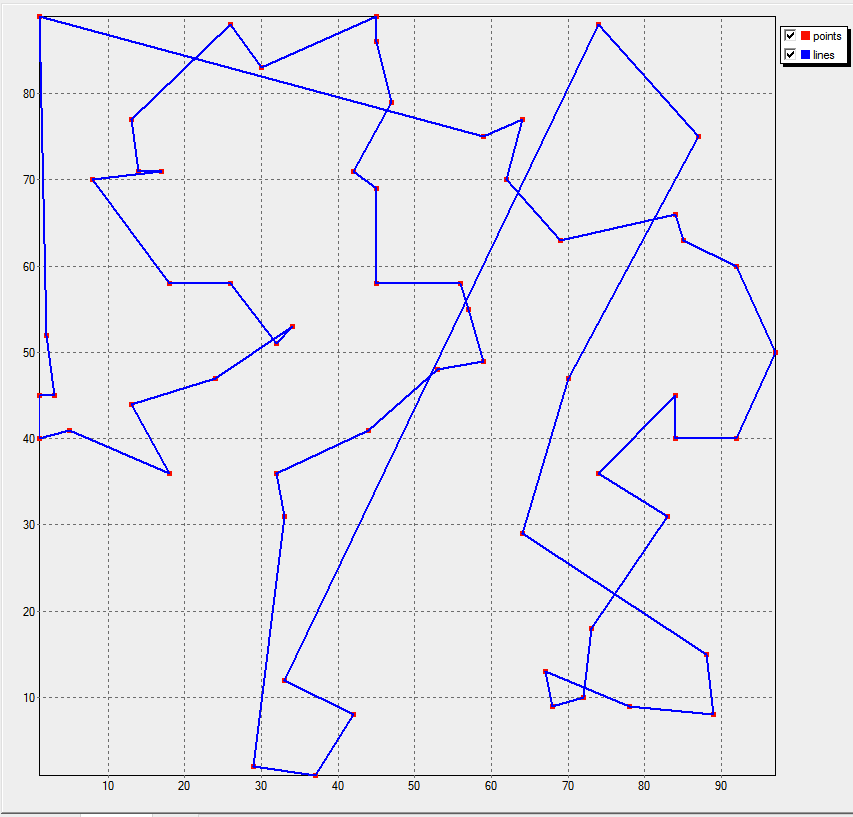
\includegraphics[width=\linewidth]{results-tsp_60_3-opt}
					\caption{Solución \emph{2-opt} para \emph{tsp\_60\_3}}
				\end{subfigure} \
				\begin{subfigure}{.4\textwidth}
					\centering
					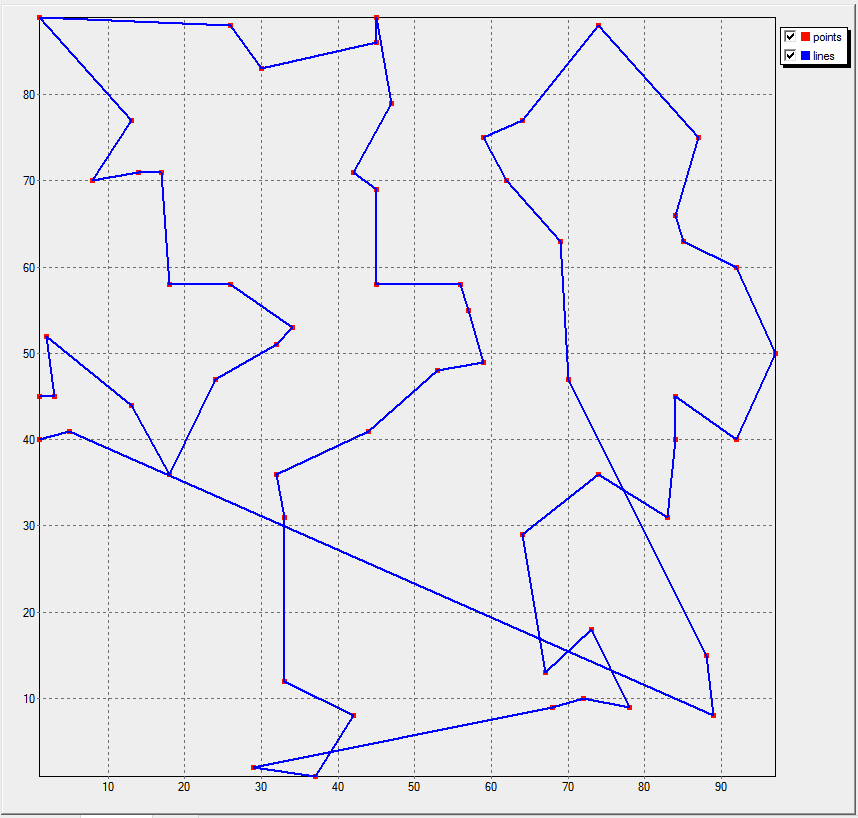
\includegraphics[width=\linewidth]{results-tsp_60_3-grasp}
					\caption{Solución \emph{GRASP} para \emph{tsp\_60\_3}}
				\end{subfigure} \\
				\begin{subfigure}{.4\textwidth}
					\centering
					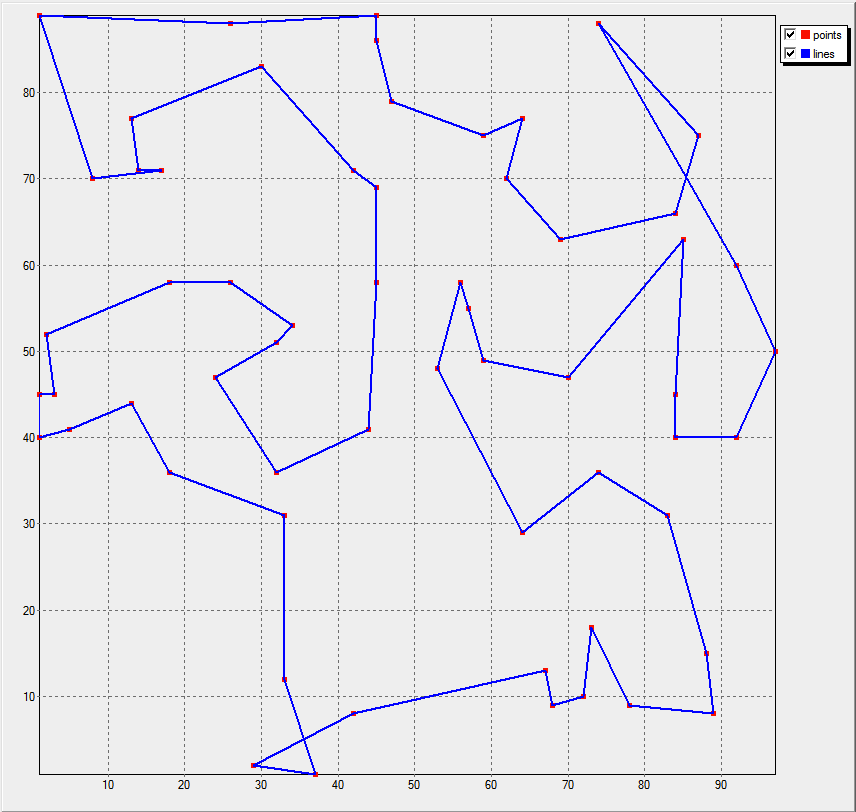
\includegraphics[width=\linewidth]{results-tsp_60_3-sa}
					\caption{Solución \emph{Simulated Anneling} para \emph{tsp\_60\_3}}
				\end{subfigure}
				\caption{Representación gráfica de las distintas soluciones para el conjunto de datos \emph{tsp\_60\_3}}
				\label{fig:sol-tsp_60_3}
			\end{figure}

		\subsection{tsp\_100\_1}

			\paragraph{}
			[TODO ]

			\begin{table}
				\centering
				\begin{tabu}{ | c | c | p{.65\linewidth} |}
					\hline
			   	\bfseries Método & \bfseries Distancia & \bfseries Camino
			    \csvreader[head to column names]{../results/csv/results-tsp_100_1.csv}{}
			    {\\\hline\method&\distance&\path}
					\\\hline
		    \end{tabu}
				\caption{Soluciones para el conjunto de datos \emph{tsp\_100\_1}}
				\label{table:sol-n21_1}
			\end{table}

			\begin{figure}[h]
				\centering
				\begin{subfigure}{.4\textwidth}
					\centering
					%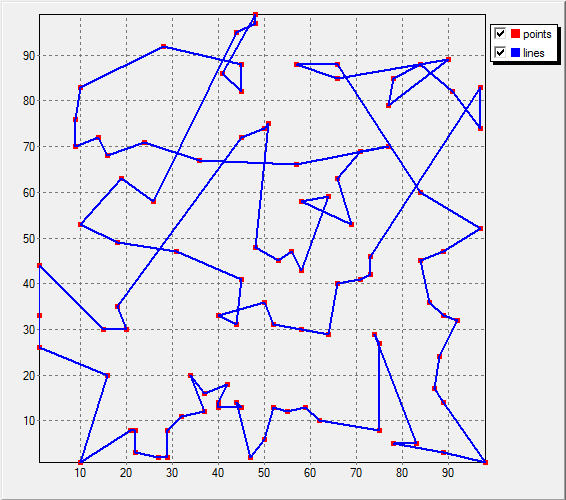
\includegraphics[width=\linewidth]{results-tsp_100_1-exact}
					\caption{Solución \emph{Exacta} para \emph{tsp\_100\_1}}
				\end{subfigure} \
				\begin{subfigure}{.4\textwidth}
					\centering
					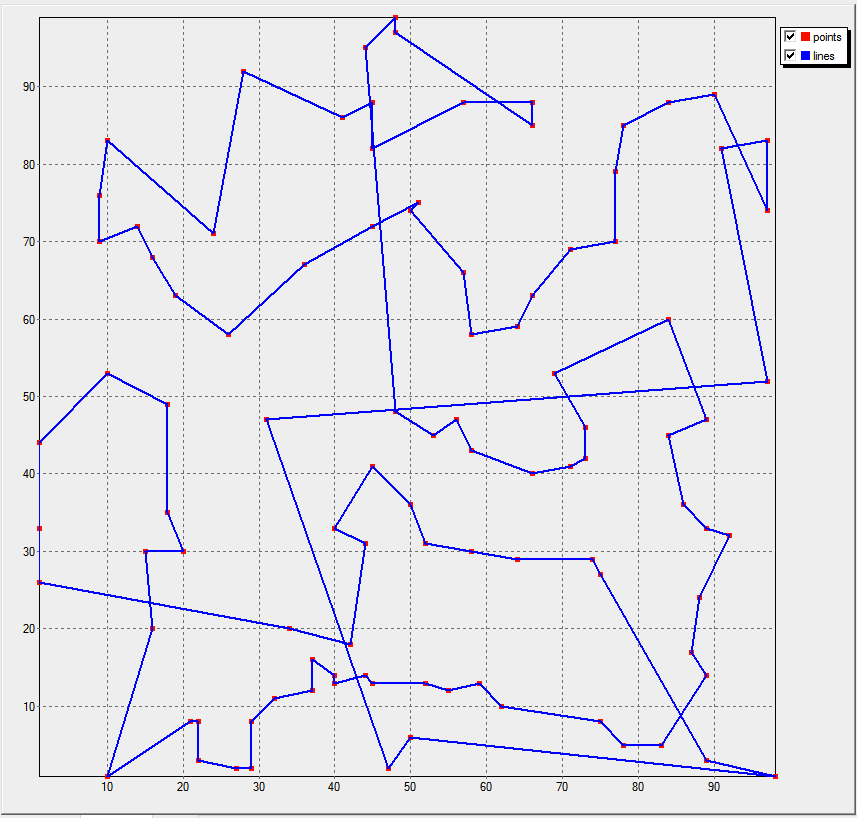
\includegraphics[width=\linewidth]{results-tsp_100_1-greedy}
					\caption{Solución \emph{Greedy} para \emph{tsp\_100\_1}}
				\end{subfigure} \\
				\begin{subfigure}{.4\textwidth}
					\centering
					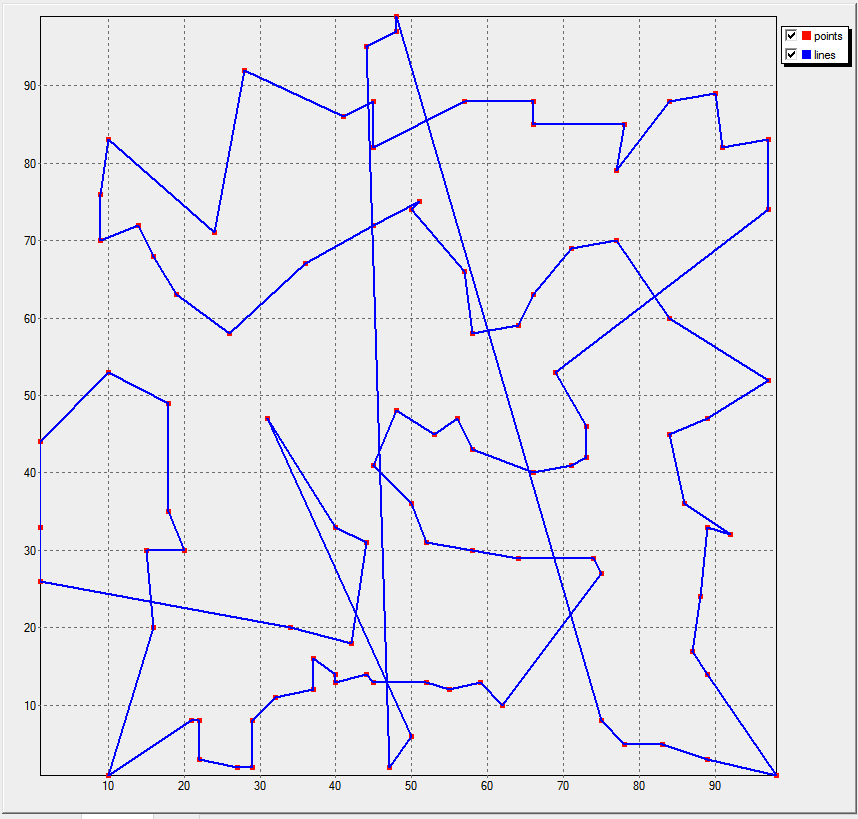
\includegraphics[width=\linewidth]{results-tsp_100_1-opt}
					\caption{Solución \emph{2-opt} para \emph{tsp\_100\_1}}
				\end{subfigure} \
				\begin{subfigure}{.4\textwidth}
					\centering
					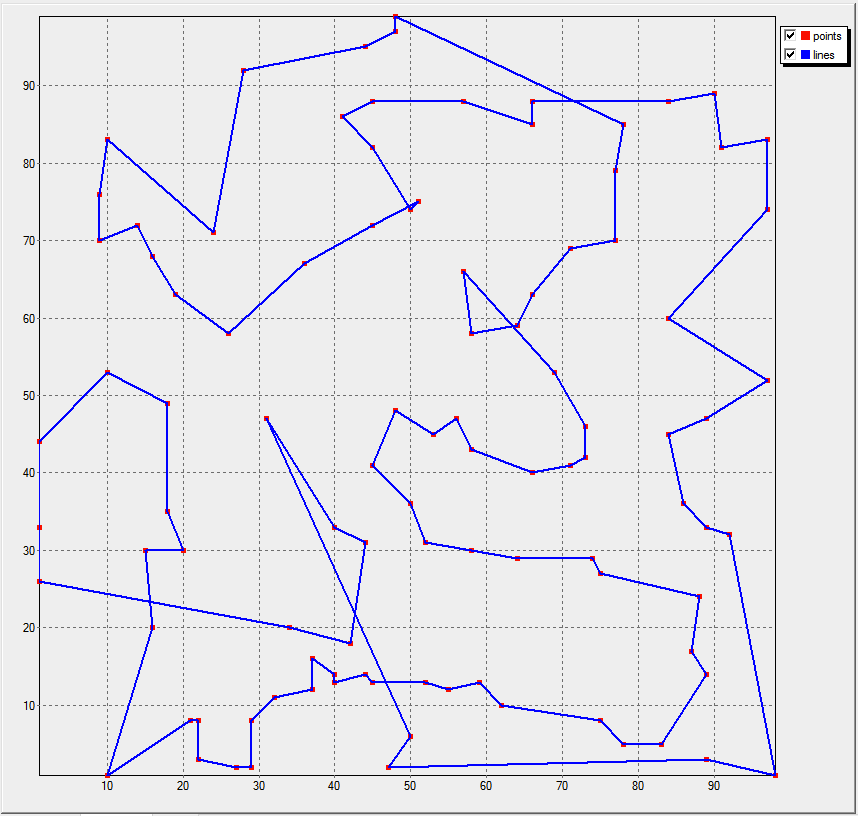
\includegraphics[width=\linewidth]{results-tsp_100_1-grasp}
					\caption{Solución \emph{GRASP} para \emph{tsp\_100\_1}}
				\end{subfigure} \\
				\begin{subfigure}{.4\textwidth}
					\centering
					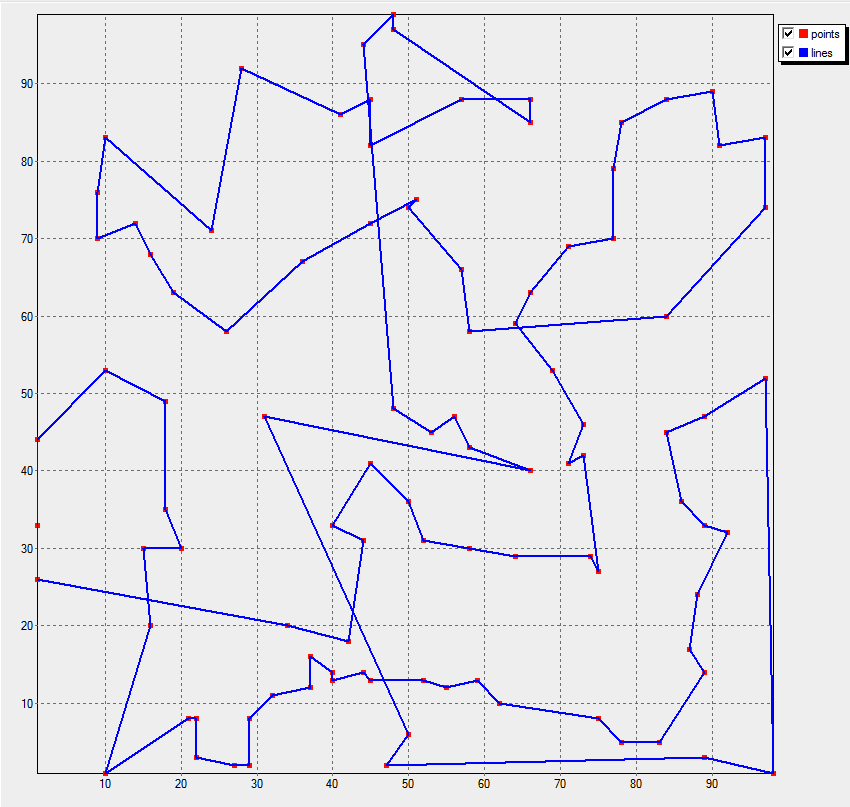
\includegraphics[width=\linewidth]{results-tsp_100_1-sa}
					\caption{Solución \emph{Simulated Anneling} para \emph{tsp\_100\_1}}
				\end{subfigure}
				\caption{Representación gráfica de las distintas soluciones para el conjunto de datos \emph{tsp\_100\_1}}
				\label{fig:sol-tsp_100_1}
			\end{figure}

		\subsection{tsp\_100\_2}

			\paragraph{}
			[TODO ]

			\begin{table}
				\centering
				\begin{tabu}{ | c | c | p{.65\linewidth} |}
					\hline
					\bfseries Método & \bfseries Distancia & \bfseries Camino
					\csvreader[head to column names]{../results/csv/results-tsp_100_2.csv}{}
					{\\\hline\method&\distance&\path}
					\\\hline
				\end{tabu}
				\caption{Soluciones para el conjunto de datos \emph{tsp\_100\_2}}
				\label{table:sol-n21_1}
			\end{table}

			\begin{figure}[h]
				\centering
				\begin{subfigure}{.4\textwidth}
					\centering
					%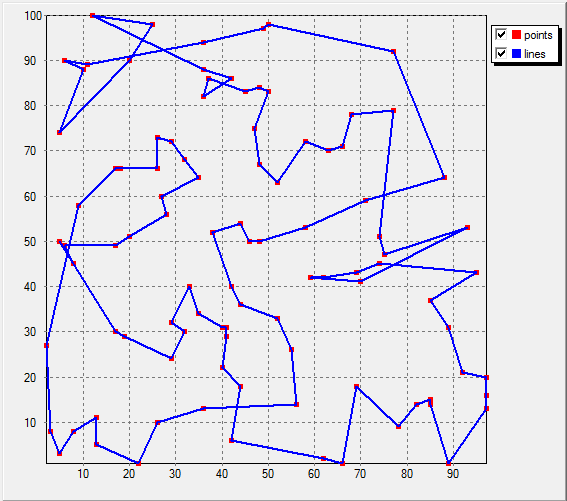
\includegraphics[width=\linewidth]{results-tsp_100_2-exact}
					\caption{Solución \emph{Exacta} para \emph{tsp\_100\_2}}
				\end{subfigure} \
				\begin{subfigure}{.4\textwidth}
					\centering
					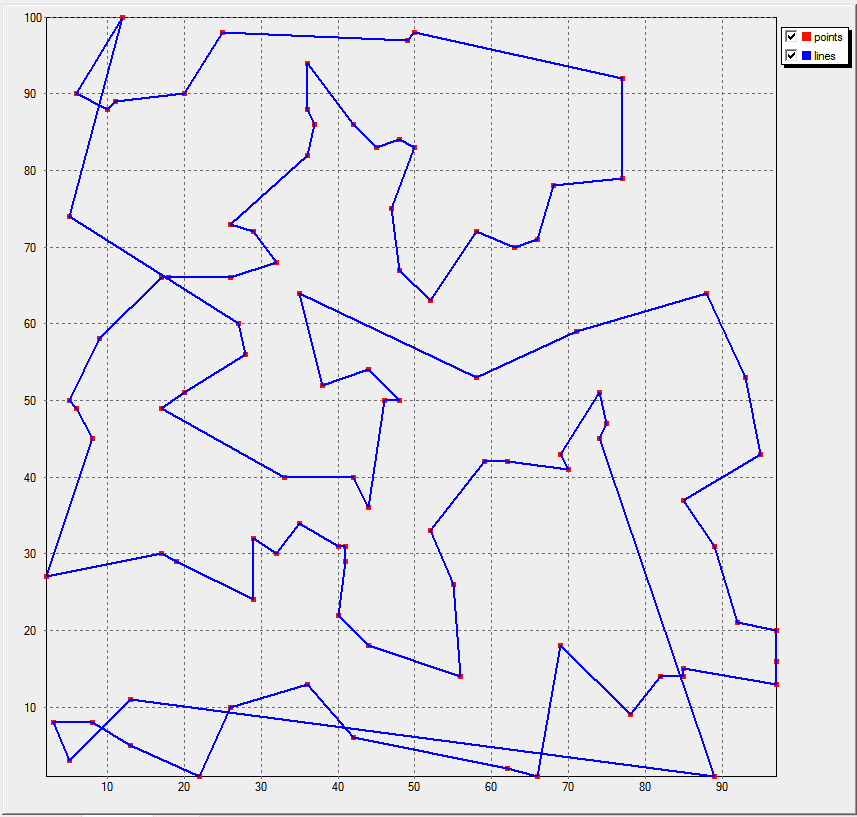
\includegraphics[width=\linewidth]{results-tsp_100_2-greedy}
					\caption{Solución \emph{Greedy} para \emph{tsp\_100\_2}}
				\end{subfigure} \\
				\begin{subfigure}{.4\textwidth}
					\centering
					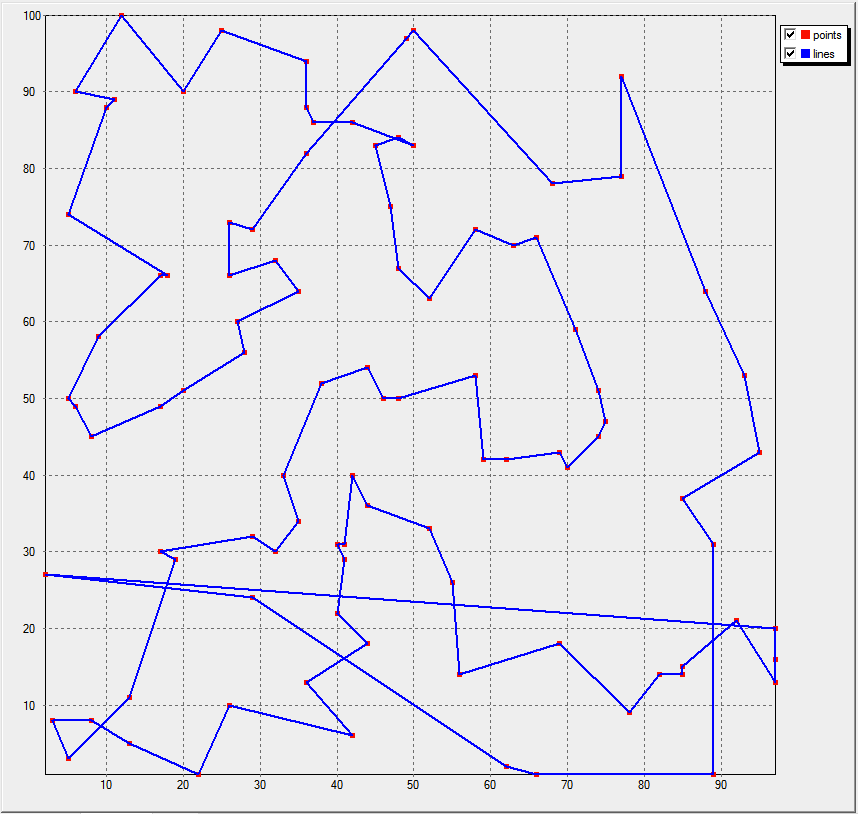
\includegraphics[width=\linewidth]{results-tsp_100_2-opt}
					\caption{Solución \emph{2-opt} para \emph{tsp\_100\_2}}
				\end{subfigure} \
				\begin{subfigure}{.4\textwidth}
					\centering
					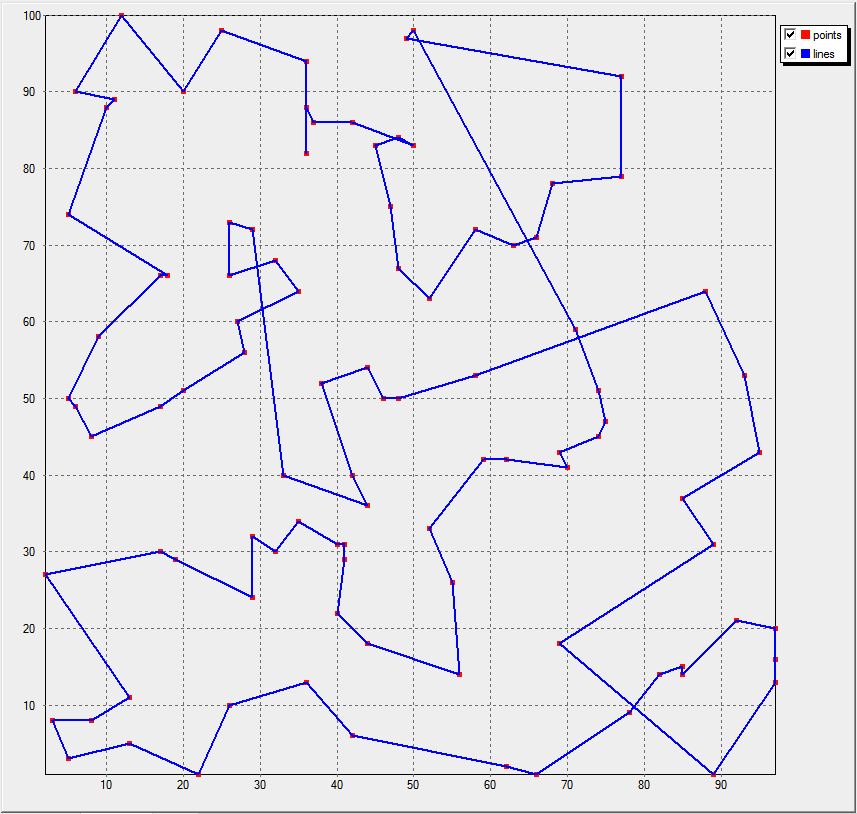
\includegraphics[width=\linewidth]{results-tsp_100_2-grasp}
					\caption{Solución \emph{GRASP} para \emph{tsp\_100\_2}}
				\end{subfigure} \\
				\begin{subfigure}{.4\textwidth}
					\centering
					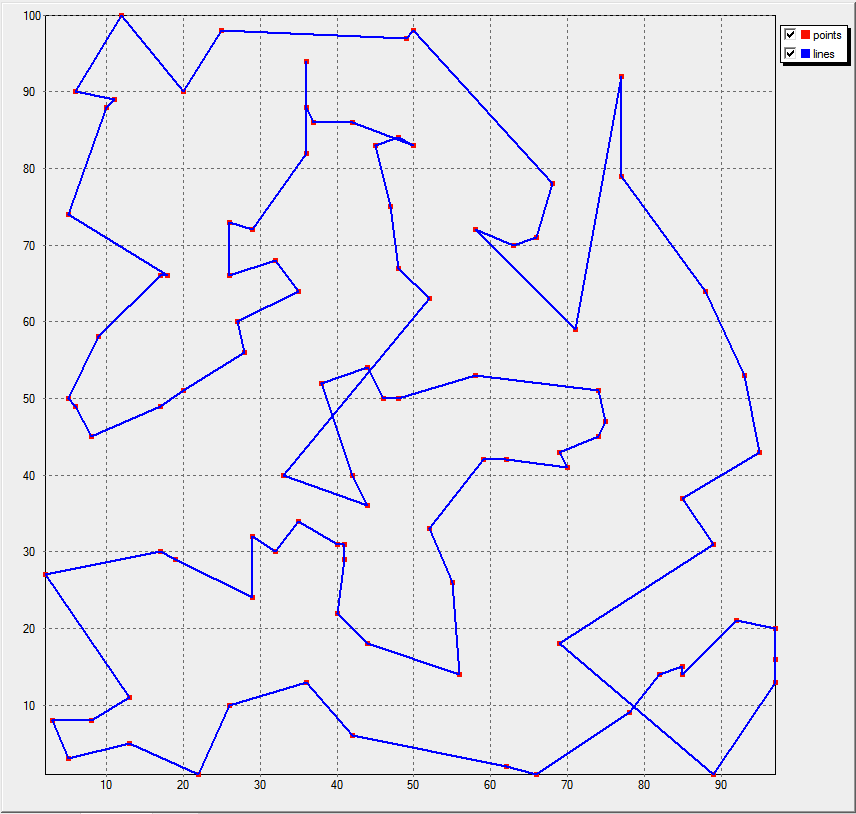
\includegraphics[width=\linewidth]{results-tsp_100_2-sa}
					\caption{Solución \emph{Simulated Anneling} para \emph{tsp\_100\_2}}
				\end{subfigure}
				\caption{Representación gráfica de las distintas soluciones para el conjunto de datos \emph{tsp\_100\_2}}
				\label{fig:sol-tsp_100_2}
			\end{figure}

		\subsection{n40w20.001}

			\paragraph{}
			[TODO ]

			\begin{table}
				\centering
				\begin{tabu}{ | c | c | p{.65\linewidth} |}
					\hline
			   	\bfseries Método & \bfseries Distancia & \bfseries Camino
			    \csvreader[head to column names]{../results/csv/results-n40w20.001.csv}{}
			    {\\\hline\method&\distance&\path}
					\\\hline
		    \end{tabu}
				\caption{Soluciones para el conjunto de datos \emph{n40w20.001}}
				\label{table:sol-n21_1}
			\end{table}

		\subsection{n40w60.004}

			\paragraph{}
			[TODO ]

			\begin{table}
				\centering
				\begin{tabu}{ | c | c | p{.65\linewidth} |}
					\hline
			   	\bfseries Método & \bfseries Distancia & \bfseries Camino
			    \csvreader[head to column names]{../results/csv/results-n40w20.004.csv}{}
			    {\\\hline\method&\distance&\path}
					\\\hline
		    \end{tabu}
				\caption{Soluciones para el conjunto de datos \emph{n40w20.004}}
				\label{table:sol-n21_1}
			\end{table}

		\subsection{n60w20.005}

			\paragraph{}
			[TODO ]

			\begin{table}
				\centering
				\begin{tabu}{ | c | c | p{.65\linewidth} |}
					\hline
			   	\bfseries Método & \bfseries Distancia & \bfseries Camino
			    \csvreader[head to column names]{../results/csv/results-n60w20.005.csv}{}
			    {\\\hline\method&\distance&\path}
					\\\hline
		    \end{tabu}
				\caption{Soluciones para el conjunto de datos \emph{n60w20.005}}
				\label{table:sol-n21_1}
			\end{table}


%-----------------------------
%	BIBLIOGRAPHY
%-----------------------------
	\nocite{subject:mio}
	\nocite{garciparedes:mosel-examples}
	\bibliographystyle{acm}
  \bibliography{bib/misc}

\end{document}
